\documentclass[main]{subfiles}

\begin{document}
    \begin{Reminder}
        \[\text{Если } f(z) = \sum_{n = 0}^\infty a_n (z - z_0)^n \]
        \[R > 0 \text{ --- рад. сх-ти}\]
        \[\forall r < R\]
        \[\text{В } \overline{D}(z_0, r) \text{ --- ст. ряд сх. равномерно}\]
        %рисунок1
        \begin{figure}[H]
            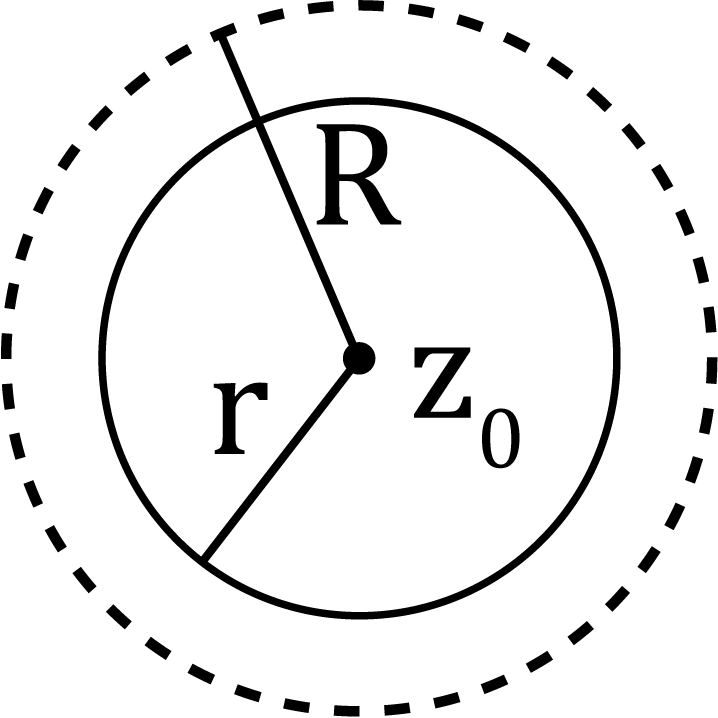
\includegraphics[width=3cm]{pics/12_1}
            \centering
        \end{figure}

        Тогда $f$ --- $\CC$ диф-ма $ \q \forall z : \abs{z - z_0} < R$
        \[f'(z) = \sum_{n = 1}^\infty a_n \cdot n (z - z_0)^{n - 1} \]
    \end{Reminder}

    \begin{Consequence}
        \[f \in C^\infty (D(z_0, R)),\q f \in H(D(z_0, R)),\q f^{(k)}(z_0) = k! a_k \]
        \[(\text{Пусть } z_0 = 0)\]
        С другой стороны
        %рисунок2
        \begin{figure}[H]
            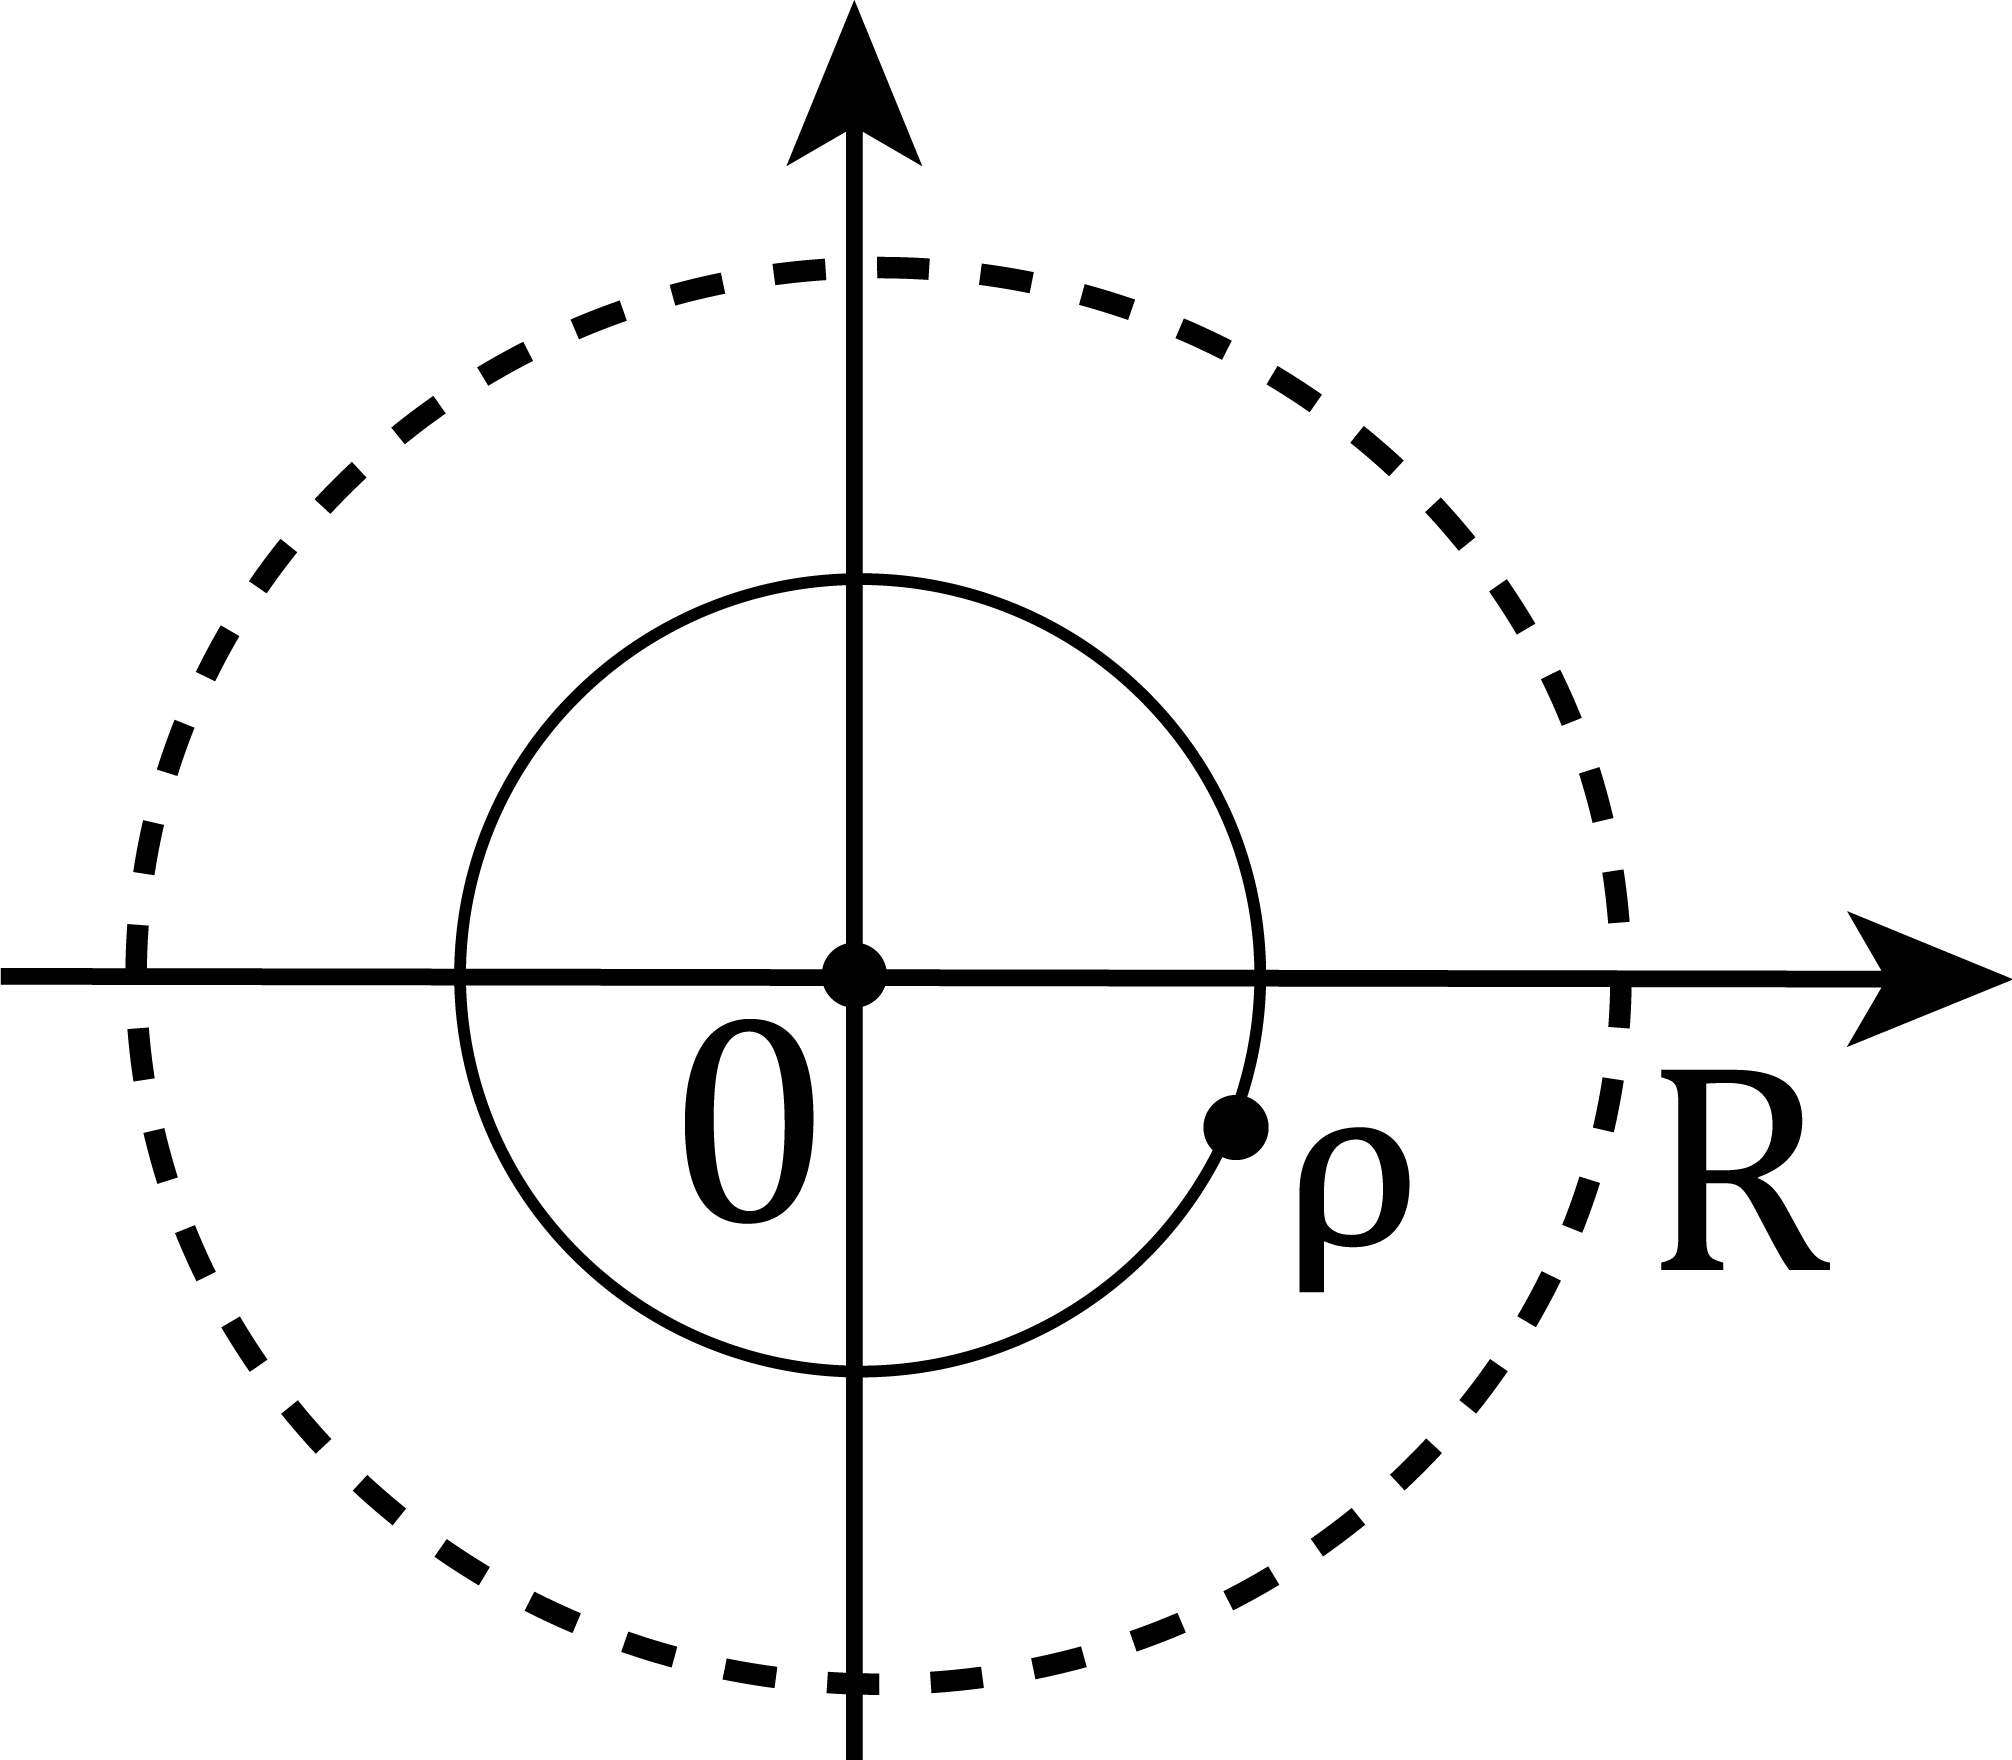
\includegraphics[width=3.5cm]{pics/12_2}
            \centering
        \end{figure}

        \[\text{Если } f \in H(D(0, R))\]
        \[\Ra (\text{в прошлый раз})\q f(z) = \sum_{k = 0}^\infty a_k z^k \]
        \[a_k = \frac{1}{2\pi i}\int_{\gamma_{\rho} } \frac{f(\xi)}{\xi^{(k + 1)} }d\xi \]
        Инт. ф. Коши
        \[f(0) = a_0 = \frac{1}{2\pi i} \int_{\gamma_{\rho} } \frac{f(\xi)}{\xi}d\xi \]

        \[\text{Если } f \in H(D(z_0, R))\]
        \[\Ra f(z) = \sum_{k = 0}^\infty a_k(z - z_0)^k \]
        \[a_k = \frac{1}{2\pi i} \int \frac{f(\xi)}{(\xi - z_0)^{k + 1} }d\xi\]
        \[\Ra \frac{1}{2\pi i} \int \frac{f(\xi)}{(\xi - z_0)^{k + 1} }d\xi = \frac{f^{(k)}(z_0) }{k!}\]
    \end{Consequence}

    \begin{Theorem}[н-ва Коши]
        \[M(\rho) = \max_{0 \leq t \leq 2\pi} \abs{f(z_0 + \rho e^{it} )} \]
        \[\abs{a_k} \leq \frac{M(\rho)}{\rho^n}\]
    \end{Theorem}

    \begin{Theorem}[основная теорема алгебры]
        \[\forall P(z) \text{ - мн-н степени } n > 0 \text{ имеет корень в } \CC\]
    \end{Theorem}

    \begin{Proof}[от противного]
        \[\text{Пусть } P(z) \neq 0 \q \forall z \in \CC\]
        \[\Ra f(z) = \frac{1}{P(z)} \in H(\CC)\]
        \[\abs{P(z)} \to \infty \qq \abs{z} \to \infty \text{ --- УПР}\]
        \[\Ra \abs{f(z)} = \frac{1}{\abs{P(z)}} \to  0 \qq \abs{z} \to \infty\]
        \[\Ra \exists R > 0:\q \forall z :\q \abs{z} > R \q \abs{f(z)} < 1\]
        %рисунок3
        \begin{figure}[H]
            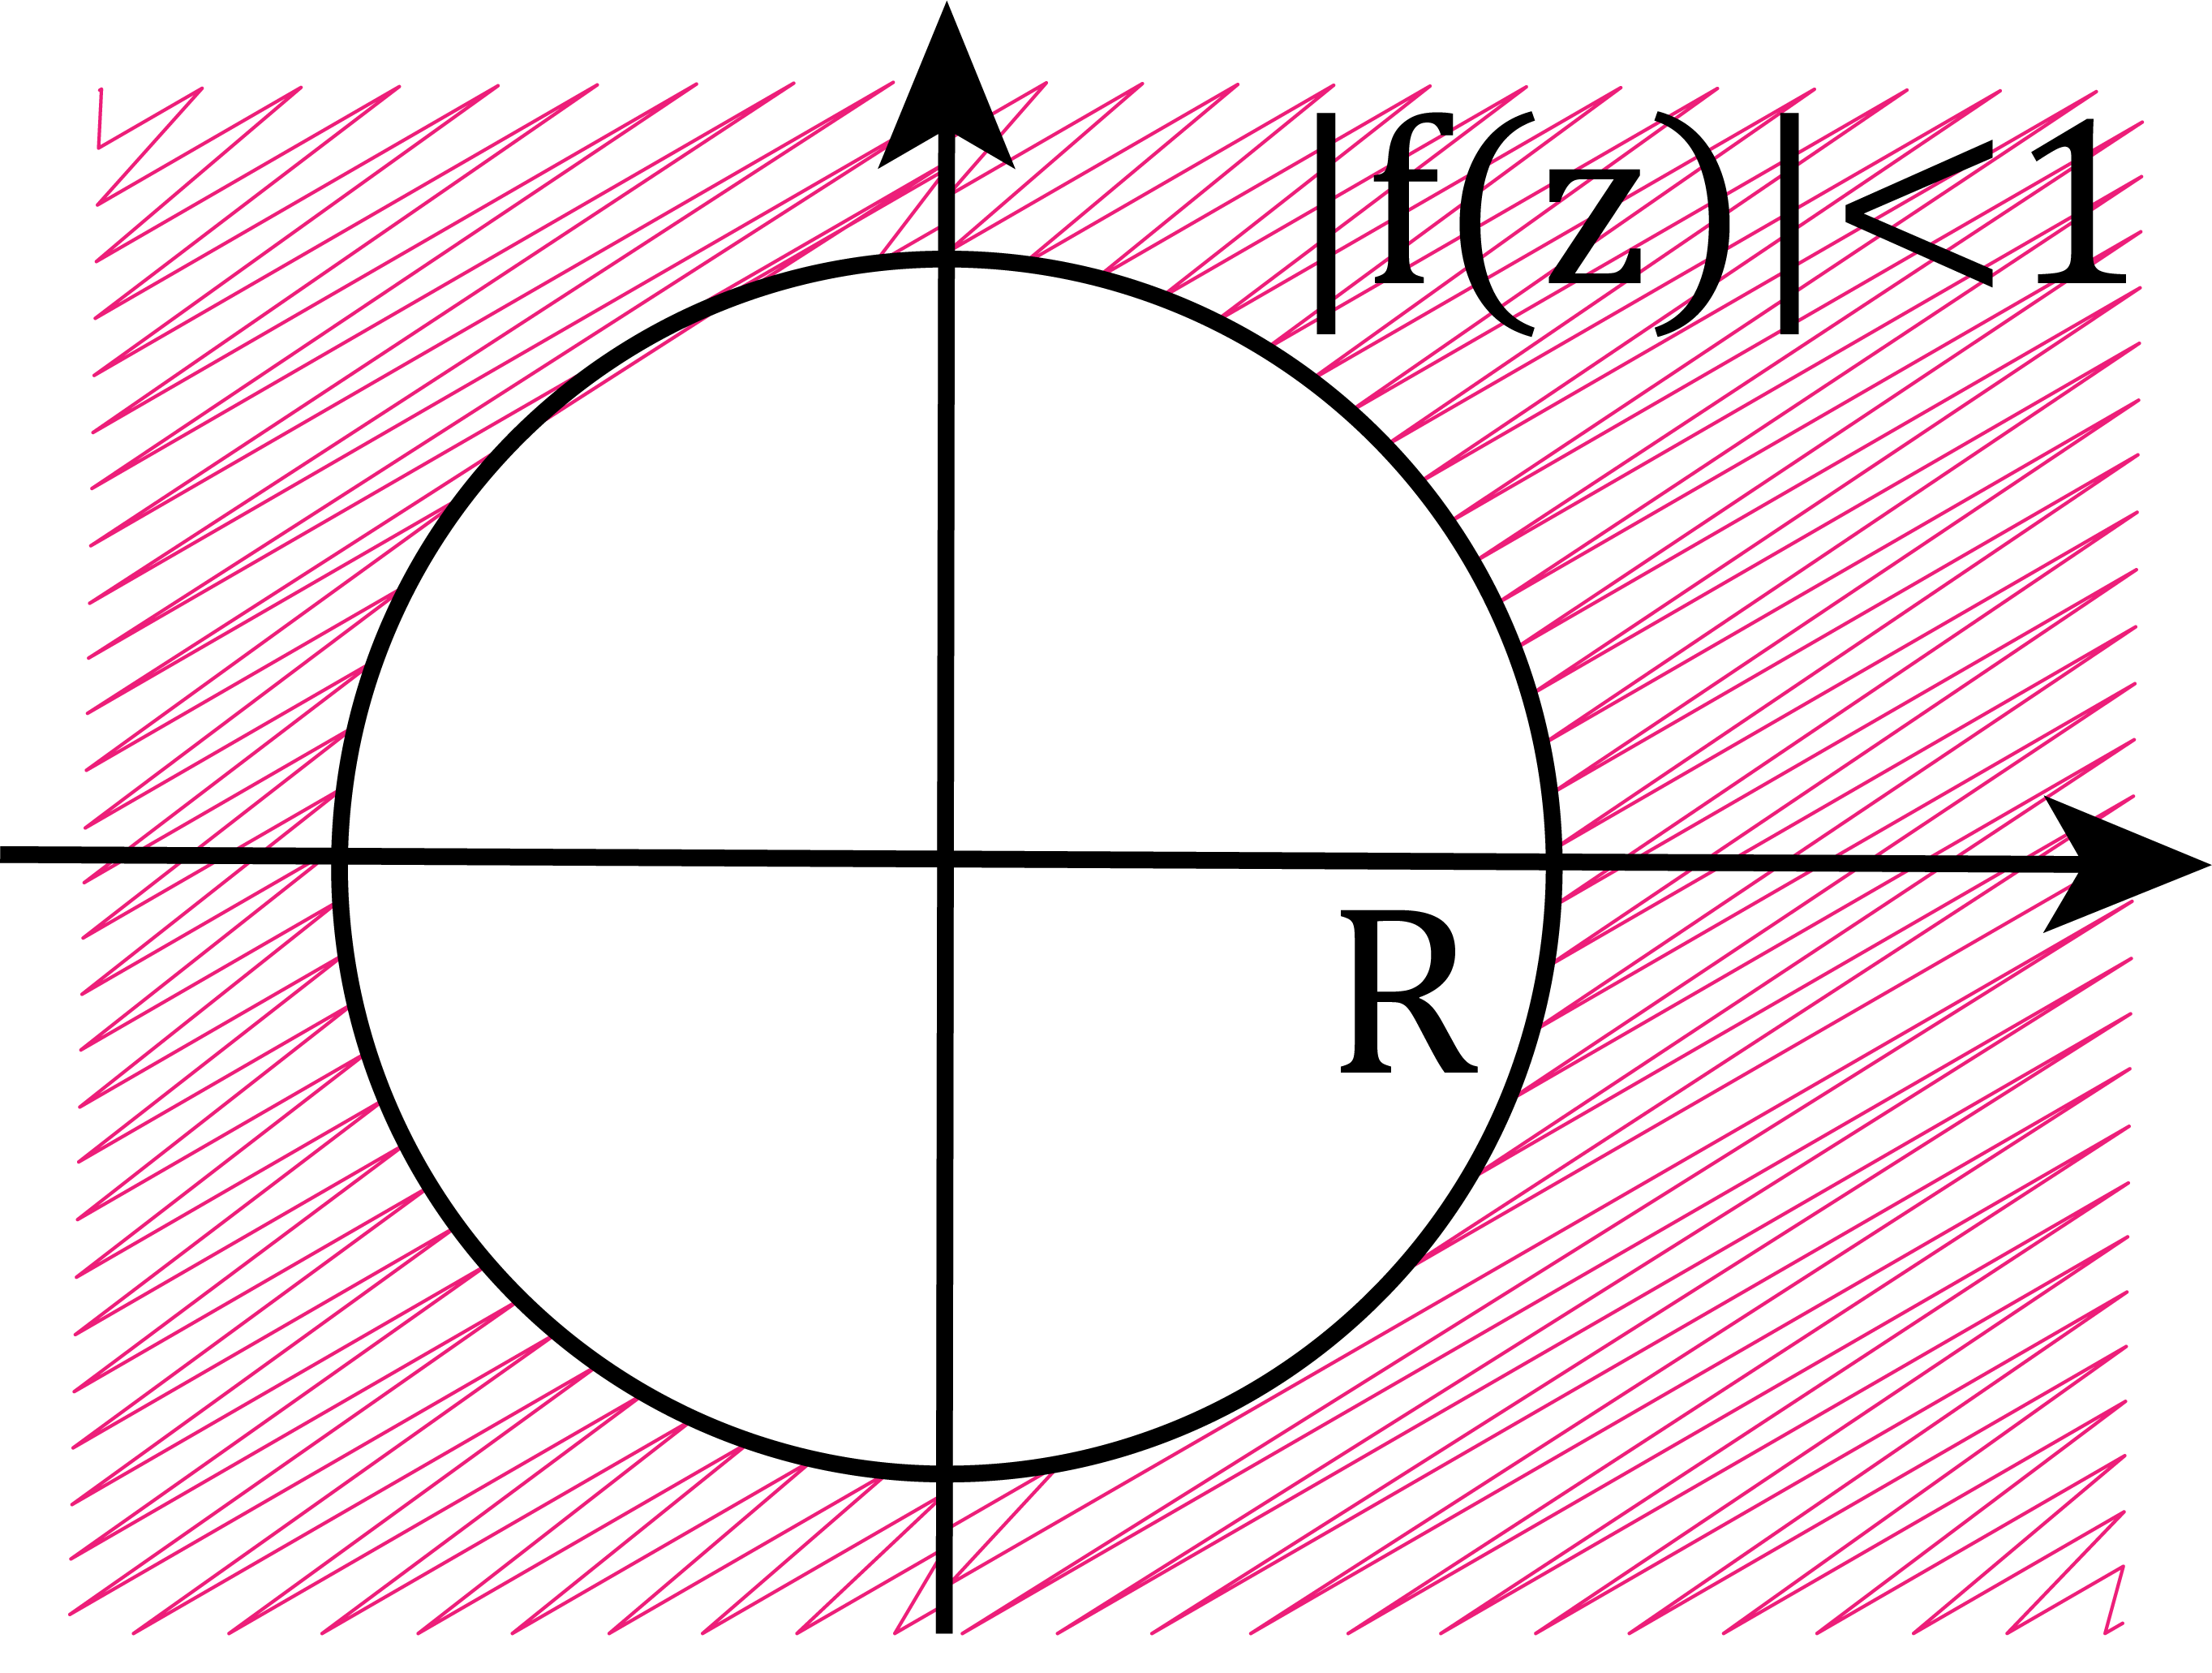
\includegraphics[width=4cm]{pics/12_3}
            \centering
        \end{figure}
        \[\text{В круге } \overline{D(0, R)},\q f(z) = \frac{1}{P(z)} \text{ (непр.)} \Ra \text{ огр.}\]
        \[\abs{f(z)} \leq M \RA \abs{f(z)} \leq \max(M, 1) \q \forall z \in \CC\]
        \[\Ra \text{ по т. Лиувилля } f(z) = \const \Ra P(z) = \const \q n = 0 \q \text{ противореч.}\]
    \end{Proof}

    \newpage
    \subsection{Теорема Мореры}

    \begin{Theorem}[Мореры]
        \[f \in C(\Omega)\]
        \[\gamma \text{ --- замк. кривая } \gamma \subset \Omega\]
        \[\text{Если } \int_{\gamma} f = 0 \q \forall \gamma \RA f \in H(\Omega) \]
    \end{Theorem}

    \begin{proof}
        По теореме (с тремя равносильными условиями)
        \[z_0 \in \Omega \text{ --- зафикс.}\]
        \[F(z) = \int_{z_0}^z f(\xi)d\xi  \text{ - явл. первообразной } \qq F'(z) = f(z)\]
        \[F \in H(\Omega) \text{ --- можем разложить в степенной ряд}\]
        \[\text{А ряд можем сколько угодно раз дифференцировать}\]
        \[\Ra f \in H(\Omega)\]
        %рисунок4
        \begin{figure}[H]
            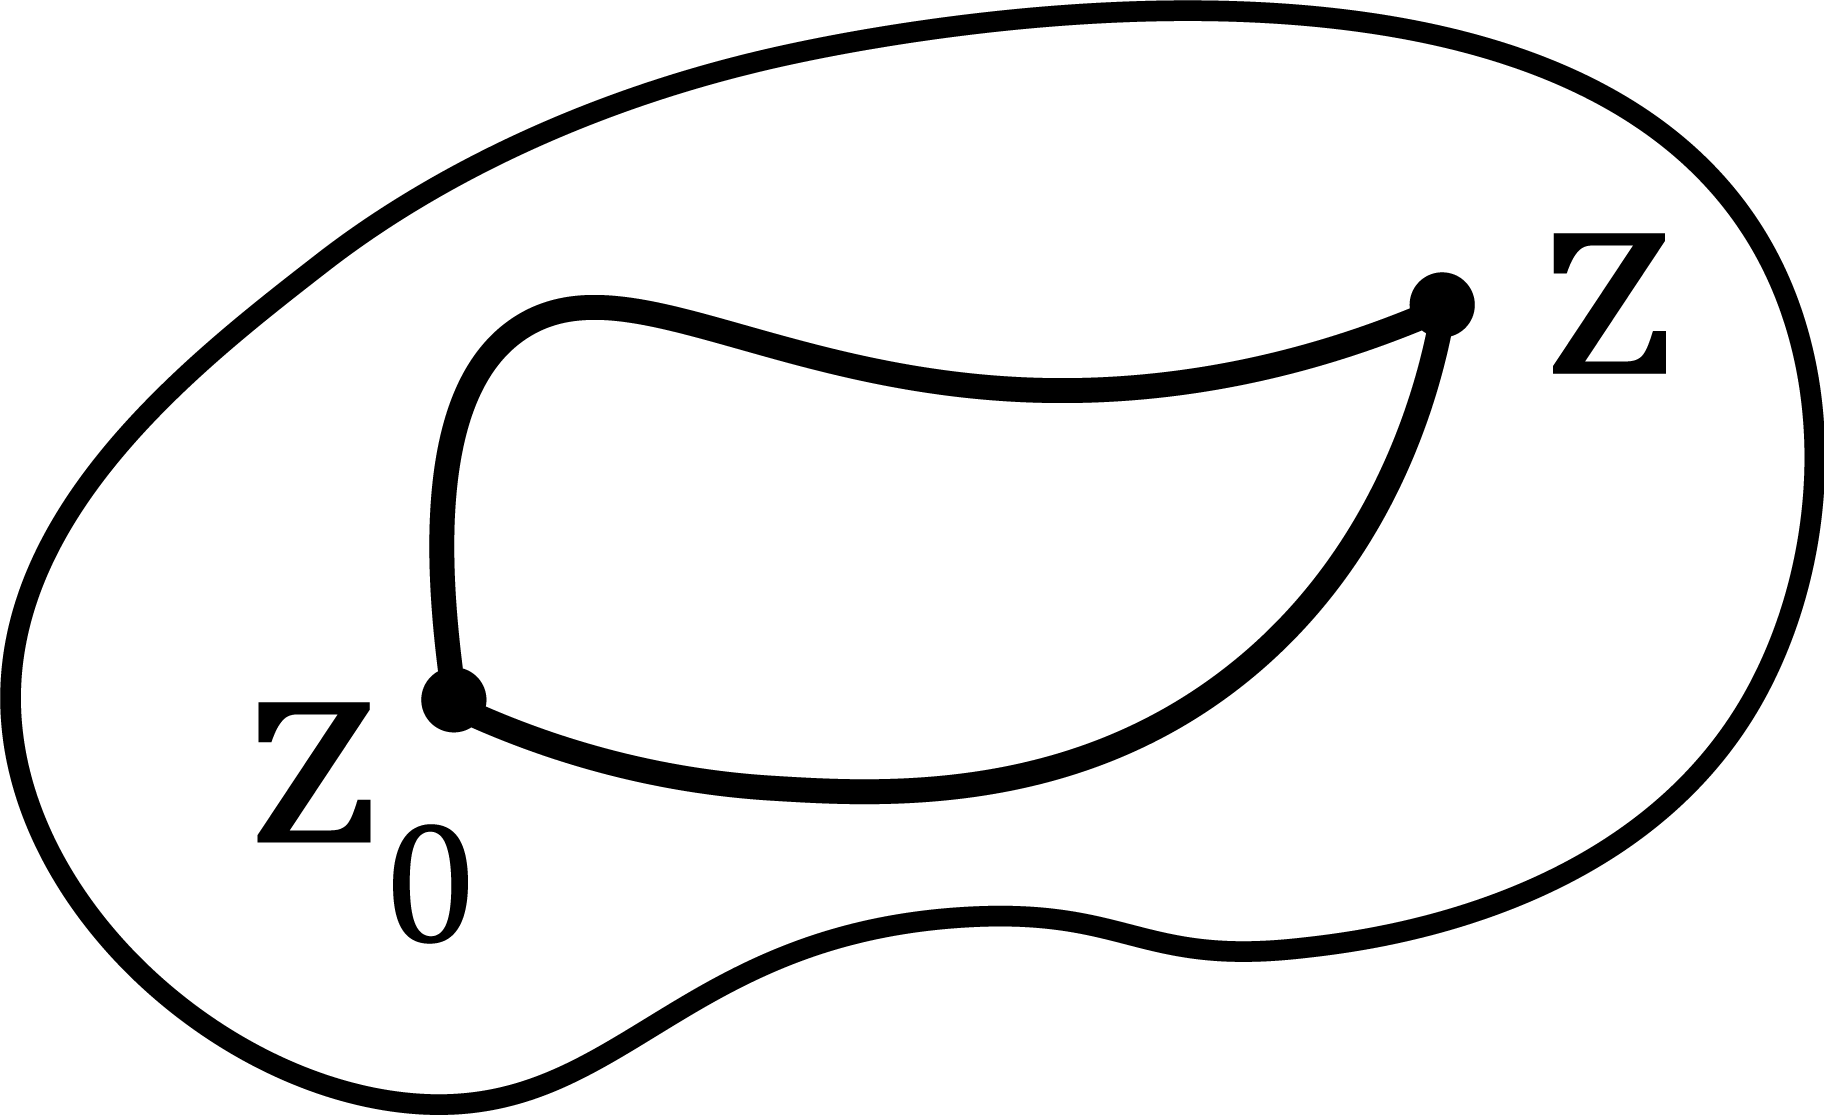
\includegraphics[width=3cm]{pics/12_4}
            \centering
        \end{figure}

    \end{proof}

    \newpage
    \subsection{Первая теорема единственности для аналитических функций}

    \begin{Theorem}[единственности аналитич. ф. №1]
        \[f \in H(\Omega) \qq z_0 \in \Omega: f^{(n)}(z_0) = 0 \qq \forall n = 0, 1 ... \]
        \[\text{Тогда } f \equiv 0 \text{ в } \Omega\]
    \end{Theorem}

    \begin{Proof}
        %рисунок5
        \begin{figure}[!h]
            
\includegraphics[width=3.5cm]{pics/12_5}
            \centering
        \end{figure}
        \[f^{(n)}(z_0) = 0 \qq \forall n = 0, 1, .. \]
        \[\text{В } D(z_0, r) \subset \Omega \q f(z) = \sum_{k = 0}^\infty \frac{f^{(k)}(z_0) }{k!}(z - z_0)^k \equiv 0\]
        \[\text{Но пока только в круге}\]
        \[\text{Соед. } z_0 \text{ и } z^*\in \Omega \text{ ломаной } L \text{  длины } l \]
        \[d = dist(L, \ \d \Omega) \]
        \[\text{Возьмем на } L \text{ точки } z_0, z_1, ..., z_n = z^* \qq z_k \in L : \abs{z_{k + 1} - z_k } <
        \frac{d}{2}\]
        %рисунок6
        \begin{figure}[!h]
            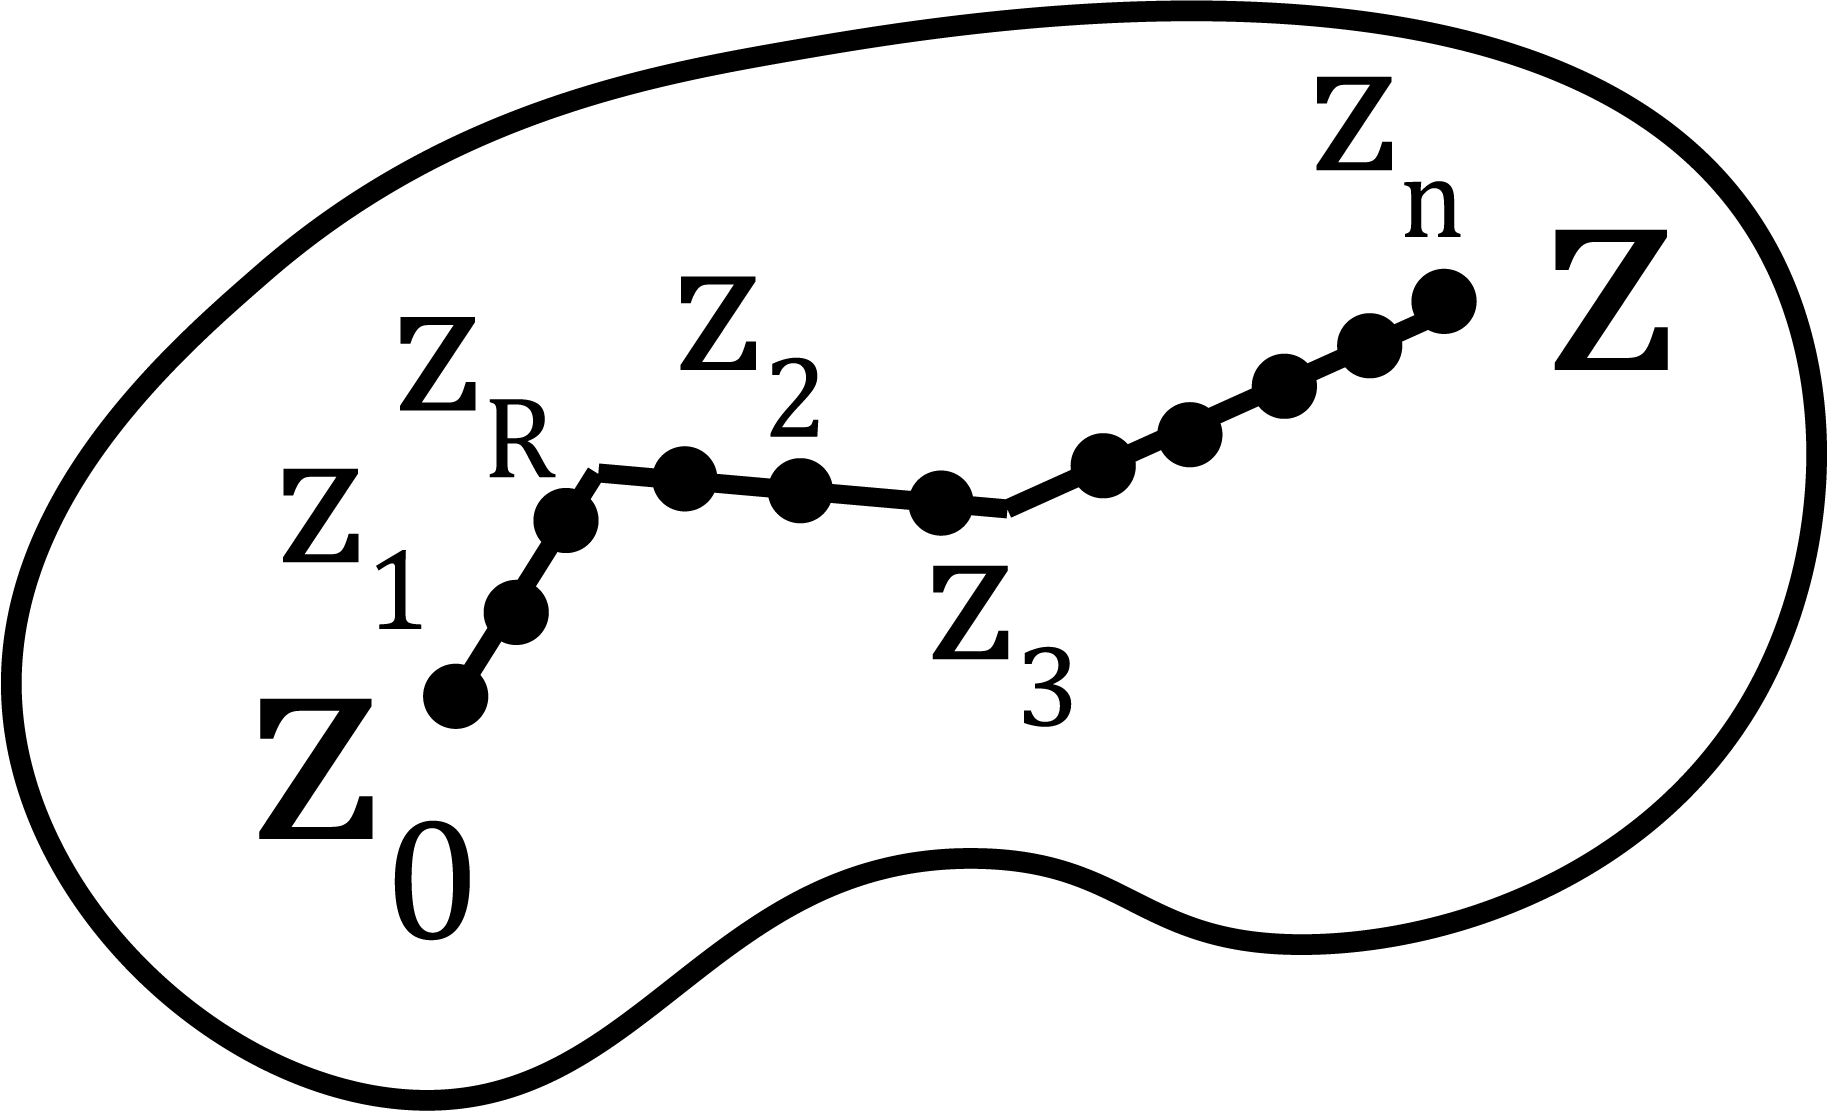
\includegraphics[width=4.5cm]{pics/12_6}
            \centering
        \end{figure}
        \[z_1 \in D(z_0, d),\q z_2 \in D(z_1, d),\q z_{k + 1} \in D(z_k, d) \]
        %рисунок7
        \begin{figure}[!h]
            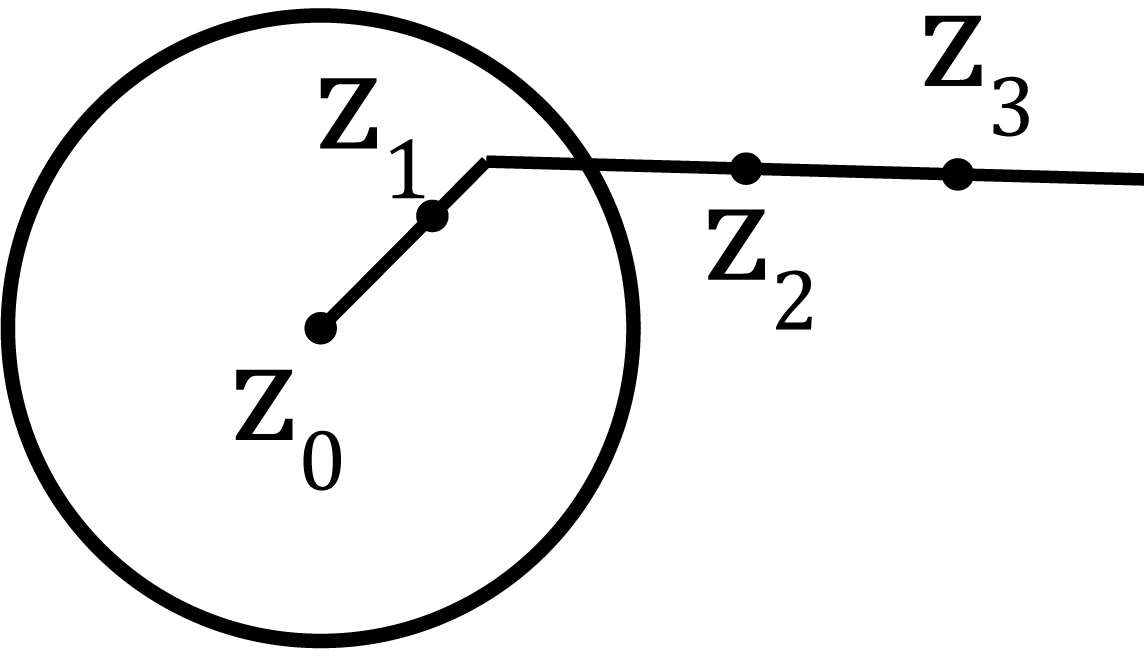
\includegraphics[width=4cm]{pics/12_7}
            \centering
        \end{figure}

        Уже показали, что $f(z) \equiv 0 \q \forall z \in D(z_0, d)$
        \[\Ra f(z_1) = 0 \text{ и } f^{(k)}(z_1) = 0 \q \forall k
        \text{ (т.к $f \equiv 0$ в круге)} \]
        \[\Ra f \equiv 0 \text{ в круге } D(z_1, d)\]
        \[\Ra f \equiv 0 \text{ в $\forall $ круге } D(z_k, d)  \Ra f(z^*) = 0\]
    \end{Proof}

    \newpage
    \subsection{Кратность  нулей  аналитической  функции.  Вторая  теорема  единственности}

    \begin{Definition}
        \[\text{Пусть } f \in H(\Omega), \q z_0 \in \Omega, \q f(z_0) = 0\]
        \[\text{Если } f(z_0) = f'(z_0) = ... = f^{m - 1}(z_0) = 0 \]
        \[f^{(m)}(z_0) \neq 0 \text{, то говорят, что }  f \text{ имеет \ul{ноль кратности $m$} в т. } z_0\]
        \[f(z) = \sum_{k = m}^\infty  \frac{f^{(k)}(z_0)} {k!} (z - z_0)^k = \]
        \[= (z - z_0)^m \underbracket{\sum_{k = m}^\infty \frac{f^{(k)}(z_0) }{k!}(z - z_0)^{k - m}}_{\varphi(z)}
        = (z - z_0)^m \cdot \varphi(z) \]
        \[\varphi(z) \in H(\Omega) \qq \varphi(z_0) \neq 0 \]
    \end{Definition}

    \begin{Theorem}[теорема единственности №2]
        \[f \in H(\Omega),\q \{z_n\}_{n = 1}^\infty \in \Omega \]
        \[z_n \us{n \to \infty}{\to } z^* \in \Omega \q z_n \neq z^* \qq \forall n \in \N\]
        \[\text{Если } f(z_n) = 0 \q \forall n \in \N \RA f(z) \equiv 0\]
    \end{Theorem}

    \begin{Example}[1]
        \[\text{Найти все } f \in H(\CC): f\Br{\frac{1}{k}} = \frac{1}{k^2} \qq \frac{1}{k} \to 0 \in \CC\]
        \[f(z) = z^2 \in H(\CC)\]
        \[\text{Пусть }\exists \widetilde{f} \in H(\CC) \qq \widetilde{f} \left(\frac{1}{k}\right) = \frac{1}{k^2}\]
        \[\text{Тогда } f \left(\frac{1}{k}\right) - \widetilde{f} \left(\frac{1}{k}\right) = 0\]
        \[f(z) - \widetilde{f}(z) \in H(\CC) \ \Ra \ f - \widetilde{f} \equiv 0\]
    \end{Example}

    \begin{Example}[2]
        \[\text{Найти } f \in H(\CC) : \q f \left(\frac{1}{k}\right) = \frac{(-1)^k}{k^2}, \q k \in \N\]
        %рисунок8
        \begin{figure}[H]
            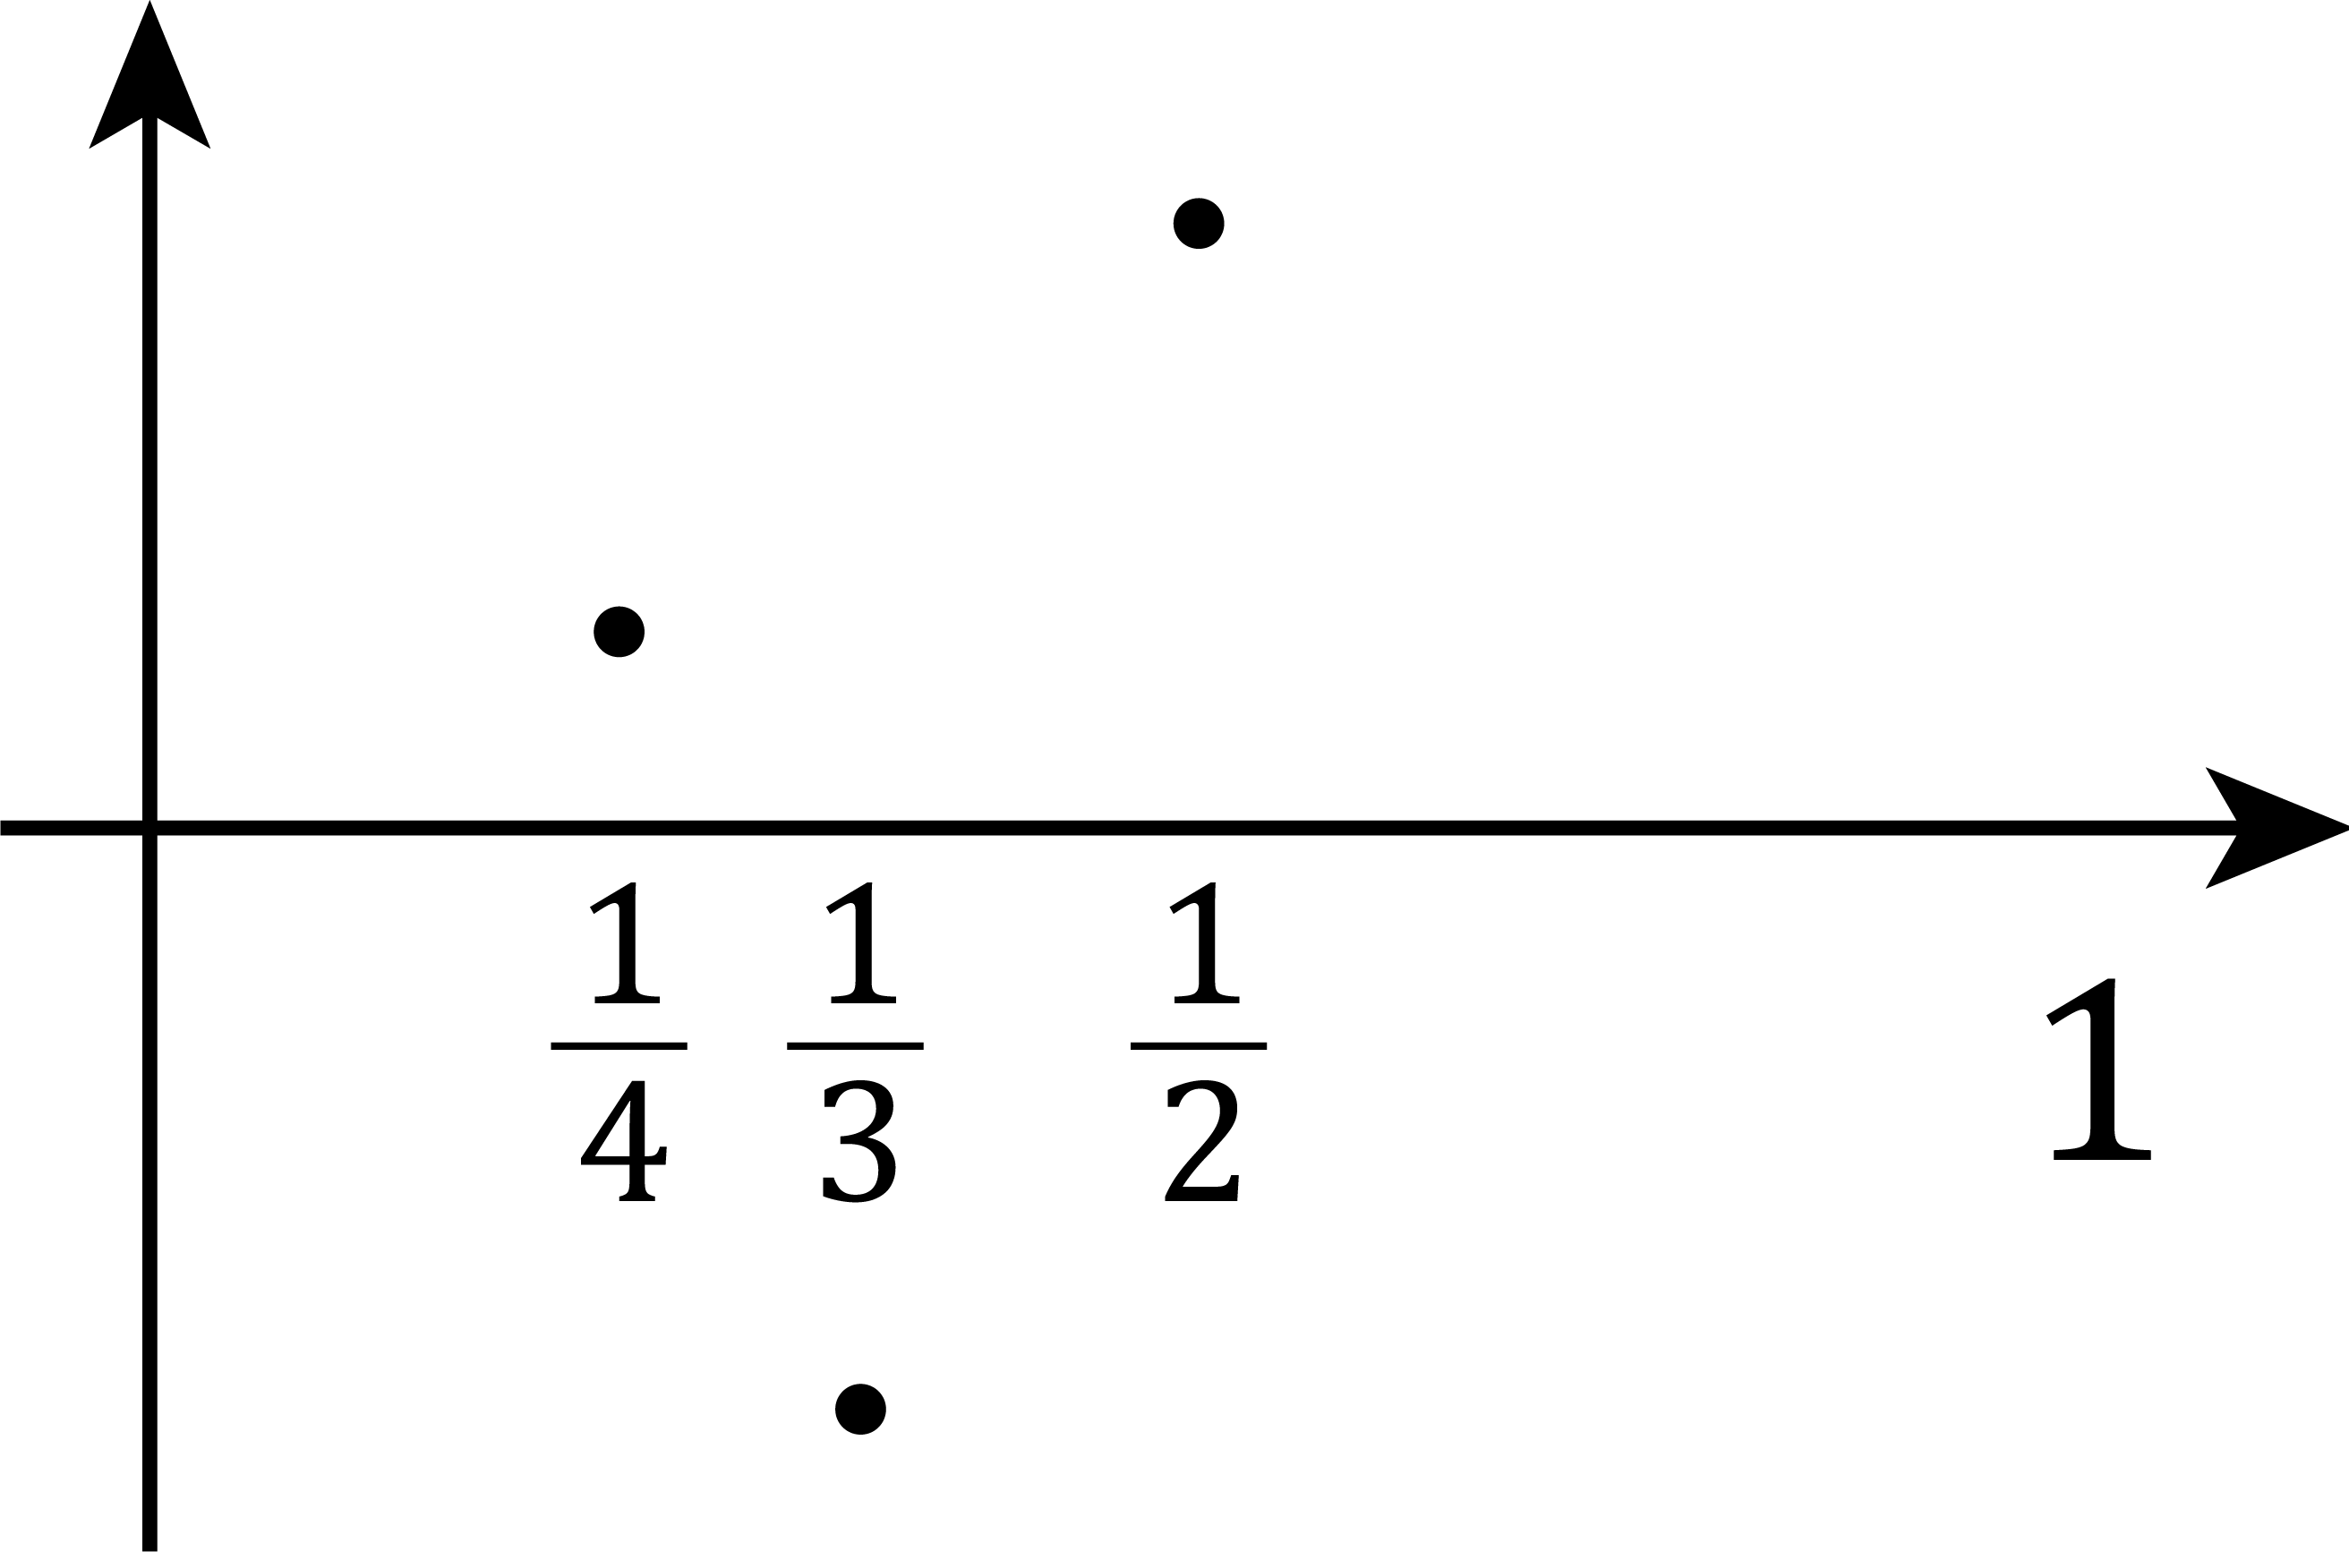
\includegraphics[width=5cm]{pics/12_8}
            \centering
        \end{figure}

        \[f\left(\frac{1}{2k}\right) = \frac{1}{(2k)^2} \text{  --- этому условию уд. } f(z) = z^2\]
        \[\Ra \forall f \in H(\CC) :\q f \left(\frac{1}{2k}\right) = \frac{1}{(2k)^2} \Ra f(z) = z^2\]
        \[\text{Но усл. } f\Br{\frac{1}{2k + 1}} = \frac{-1}{(2k + 1)^2} \text{ она не уд. $\Ra$ таких ф. нет}\]
    \end{Example}

    \begin{Example}[3]
        \[f(z) = \sin^2 z + \cos^2 z \in H(\CC)\]
        \[\forall z \in \R \q f(z) = 1\]
        \[f(z) - 1 = 0 \q \forall z \in \R, \text{ в частности для } z_k = \us{\in \R}{\frac{1}{k}} \to 0\]
        \[\Ra f(z) - 1 = 0 \q \forall z \in \CC \text{ по т. ед. №2}\]
    \end{Example}

    \begin{Consequence}
        \[f, g \in H(\Omega),\q G \subset \Omega\]
        \[G \text{ - беск., имеет т. сгущ. (т. е. $\exists z_k \in G : z_k \to z^* \in G,
        z_k \neq z^*$)}\]
        \[\text{Если } f\big|_G = g\big|_G \Ra f(z) = g(z) \q \forall z \in \Omega\]
    \end{Consequence}

    \begin{Proof}[т. ед. №2]
        \[f(z_k) = 0 \q \forall k \qq f \in H(\Omega) \subset C (\Omega)\]
        \[\Ra \lim_{k \to \infty} f(\os{=0}{z_k}) = f(z^*) = 0 \]
        \[z_k \to z*\]
        \[\text{Т.о. } z^* \text{ --- ноль } f(z)\]
        \[\text{Пусть } z^* \text{ --- ноль }f \text{ кратности } m \geq 1\]
        \[f(z^*) = f'(z^*) = ... = f^{(m - 1)}(z^*) = 0 \]
        \[f(z) = (z - z^*)^m \varphi(z) \qq \varphi \in H(\Omega)\]
        \[0 = f(z_k) = (\ub{\neq 0}{z_k - z^*})^m \varphi(z_k)\]
        \[\Ra \varphi(z_k) = 0 \q \forall k \Ra \varphi(z^*) = 0\]
        \[\Ra \varphi(z^*) = \frac{f^{(m)}(z^*) }{m!} = 0 \text{ и т.д. по инд.}\]
        \[\Ra f^{m}(z^*) = 0 \q \forall m \in \N \Ra \text{ по т. ед №1} \q f(z)
        \equiv 0 \q \forall z \in \Omega \]
    \end{Proof}

    \newpage
    \subsection{Принцип максимума модуля аналитических функций}

    \begin{Theorem}[принцип максимума модуля аналит. функции]
        \[f \in H(\Omega), \q z_0 \in \Omega\]
        \[\text{Если }\abs{f(z_0)} \geq \abs{f(z)}\q \forall  z \in \Omega \Ra f(z) \equiv \const\]
        \[\text{(макс. модуля аналит. ф-ии не может достигаться во внутр. точке)}\]
    \end{Theorem}

    \begin{consequence}
       Модуль аналит. ф-ии не может иметь локального $\max$ во внутр точке области аналитичности,
       если $f \neq \const$
       %рисунок9
       \begin{figure}[H]
           
\includegraphics[width=3cm]{pics/12_9}
           \centering
       \end{figure}

    \end{consequence}

    \begin{Proof}[следствия]
        \[f \in H(\Gamma),\q \letus z_0 \text{ --- т. лок. }\max \ |f(z)|\]
        \[\Ra \e U(z_0) \subset \Gamma: |f(z_0)| \geq |f(z)| \q \forall z \in U(z_0)\]
        \[\Ra \text{ по т. $f(z) = \const$ в $U(z_0)$}\]
        \[\Ra \text{ по т. ед №2 $f(z) = \const$ в } \Omega\]
    \end{Proof}

    \begin{Proof}[теоремы]
        \[\letus r: \q \gamma_r : z = z_0 + re^{it} \]
        \[\overline{D(z_0, r)} \subset \Omega\]
        \[\text{По т. о среднем } f(z_0) = \frac{1}{2\pi}\int_{-\pi}^\pi f(z_0 + re^{it} )dt \]
        \[M = \abs{f(z_0)} = \frac{1}{2\pi} \abs{\int_{-\pi}^\pi f(z_0 + re^{it} )dt } \leq
        \frac{1}{2\pi} \int_{-\pi}^\pi  \abs{f(z_0 + re^{it} )}dt\]
        \[\int_{-\pi}^\pi (\abs{f(z_0 + re^{it}) } - M) dt \geq 0 \RA \abs{f(z_0 + re^{it} )} - M \leq 0\]
        \[\Ra \int_{-\pi}^\pi (\abs{f(z_0 + re^{it} )} - M)dt = 0 \RA \abs{f(z_0 + re^{it} )} = M\]
        \[\text{Это верно } \forall 0 < \rho < r\]
        \[\text{В $D(z_0, r)$:}\q \abs{f} \equiv const \Ra f \equiv \const \text{ в } D(z_0, r) \subset \Omega\]
        \[\Ra f \equiv \const \text{ в $\Omega$ (по т. ед.)}\]
    \end{Proof}

    \newpage
    \subsection{Ряд Лорана, его область сходимости. Теорема Лорана. Неравенства Коши}

    \begin{Example}
        \[\frac{1}{(z - 1)(z - 2)} = \frac{1}{z - 2} - \frac{1}{z - 1}\]
        %рисунок10
        \begin{figure}[H]
            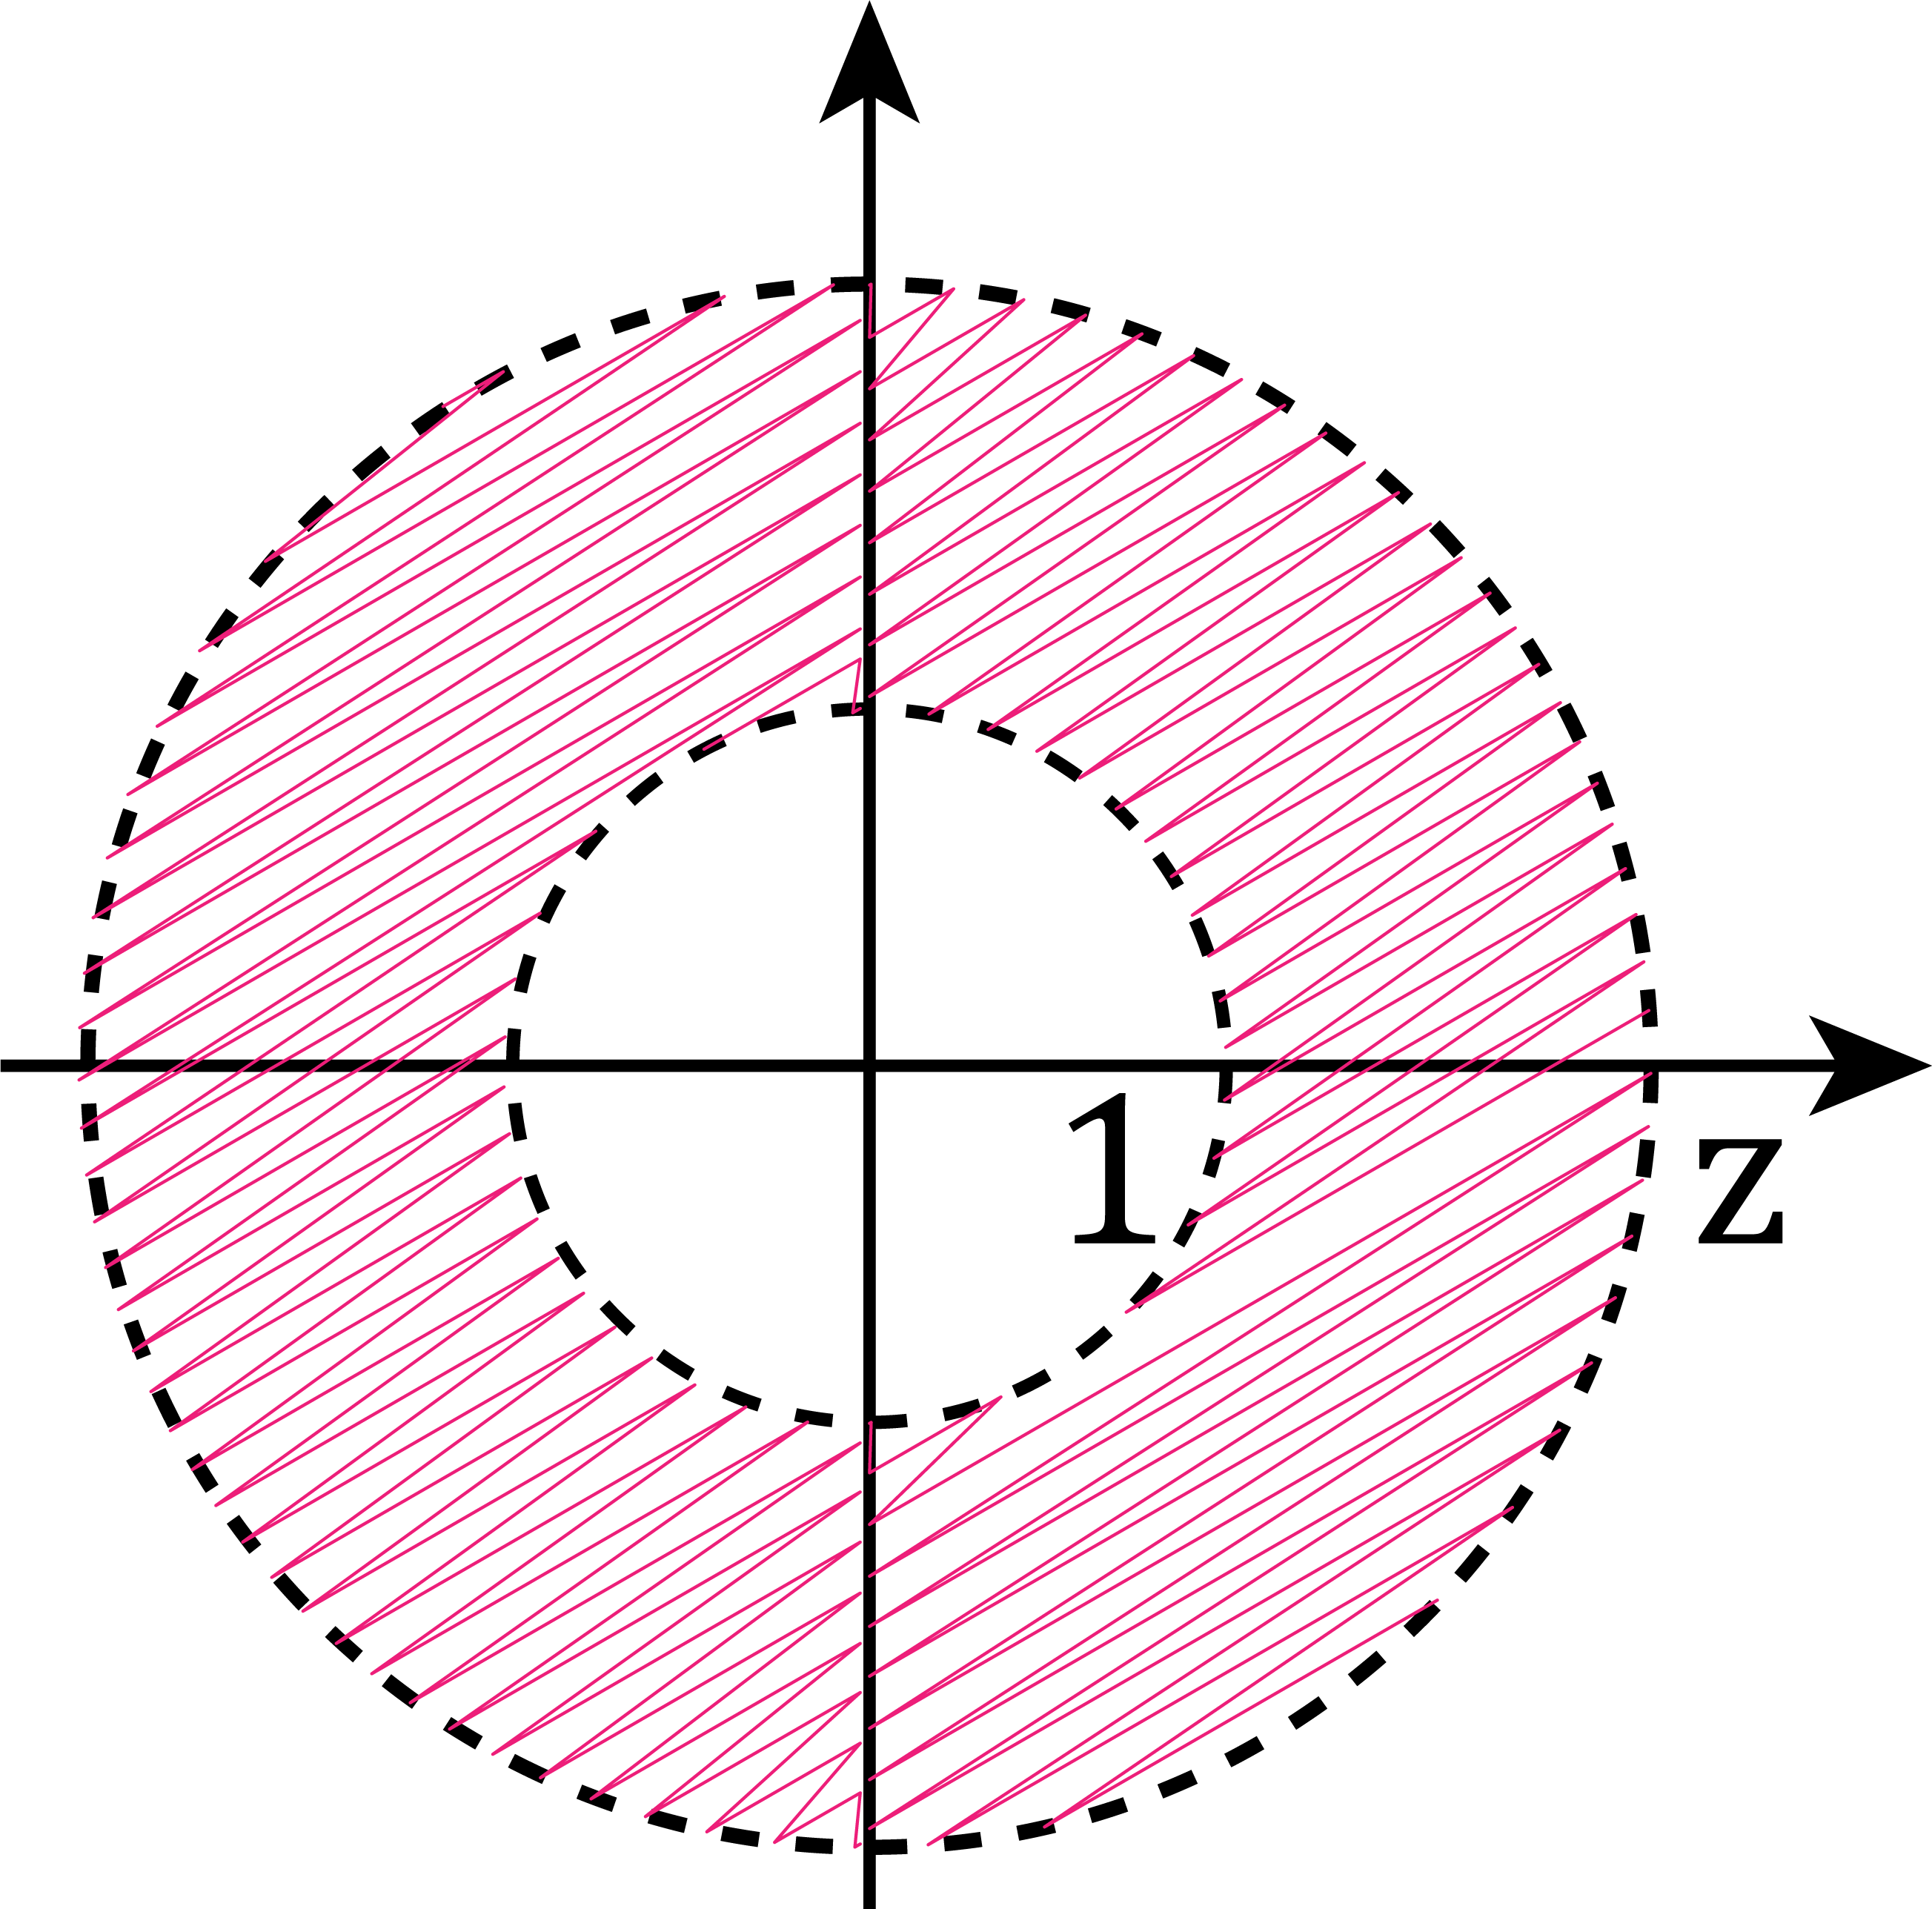
\includegraphics[width=5cm]{pics/12_10}
            \centering
        \end{figure}

        \[\text{в } 1 < \abs{z} < 2\]
        \[\frac{1}{z - 2} = \frac{1}{2} \cdot \frac{1}{\frac{z}{2} - 1} = - \frac{1}{2}\sum_{n = 0}^\infty \left(\frac{z}{2}\right)^n\]
        \[\Br{\abs{z} < 2 \Ra \abs{\frac{z}{2}} < 1}\]
        \[\frac{1}{z - 1} = \frac{1}{z} \cdot \frac{1}{1 - \frac{1}{z}} = \frac{1}{z}\sum_{n = 0}^\infty \frac{1}{z^n} = \sum_{n = 0}^\infty \frac{1}{z^{n + 1}} \]
        \[\Br{\abs{z} > 1\ \Ra \frac{1}{\abs{z}} < 1}\]
        \[\frac{1}{(z-1)(z-2)} = \us{\text{пол. степени}}{ -\frac{1}{2}\sum_{n = 0}^\infty \frac{z^n}{2^n}}
        - \us{\text{отр. степени}}{\sum_{n = -1}^{-\infty}z^n}  \qq 1 < \abs{z} < 2\]
    \end{Example}

    \begin{Definition}[ряд Лорана]
        \[\sum_{k = -\infty}^\infty c_k(z - z_0)^k = \sum_{k \geq 0} c_k (z - z_0)^k +
        \sum_{k < 0} c_k (z - z_0)^k \]
        \[\sum^+ = \sum_{k \geq 0} c_k (z - z_0)^k \qq \q \abs{z - z_0} < R \text{ обл сх.} \]
        \[\sum^- = \sum_{k < 0} c_k (z - z_0)^k = \sum_{n = 1}^{+\infty} \frac{c_k}{(z - z_0)^n}   \]
        \[\frac{1}{z - z_0} = w \qq \sum_{k = 1}^\infty c_k w^k \]
        \[\text{Обл сх. } \abs{w} < R_-\]
        По формуле Коши-Адамара
        \[\abs{z - z_0} < R_+ = \frac{1}{\overline{\displaystyle \lim_{k \to \infty} }\sqrt[k]{c_k}} \]
        \[\abs{z - z_0} > \frac{1}{R_-} = r_-\]
        \[\text{Т.о. } \sum_+ \text{ сх в } \abs{z - z_0} < R_+\]
        \[\sum_- \text{ в } \abs{z - z_0} > r_-\]
        \[\text{Если } R_+ < r_- \text{ --- нет общей обл. сх.}\]
        \[ \us{\abs{z} < 1}{\sum_{n = 0}^\infty z^n }+ \us{\abs{z} > 1}{\sum_{n = 1}^\infty \frac{1}{z^n}} \q\text{нигде не сходится} \]
        \[\text{Если } r < R\]
        \[\text{Обл. сх ряда Л. } r < \abs{z - z_0} < R \text{ кольцо} \]
        %рисунок11
        \begin{figure}[H]
            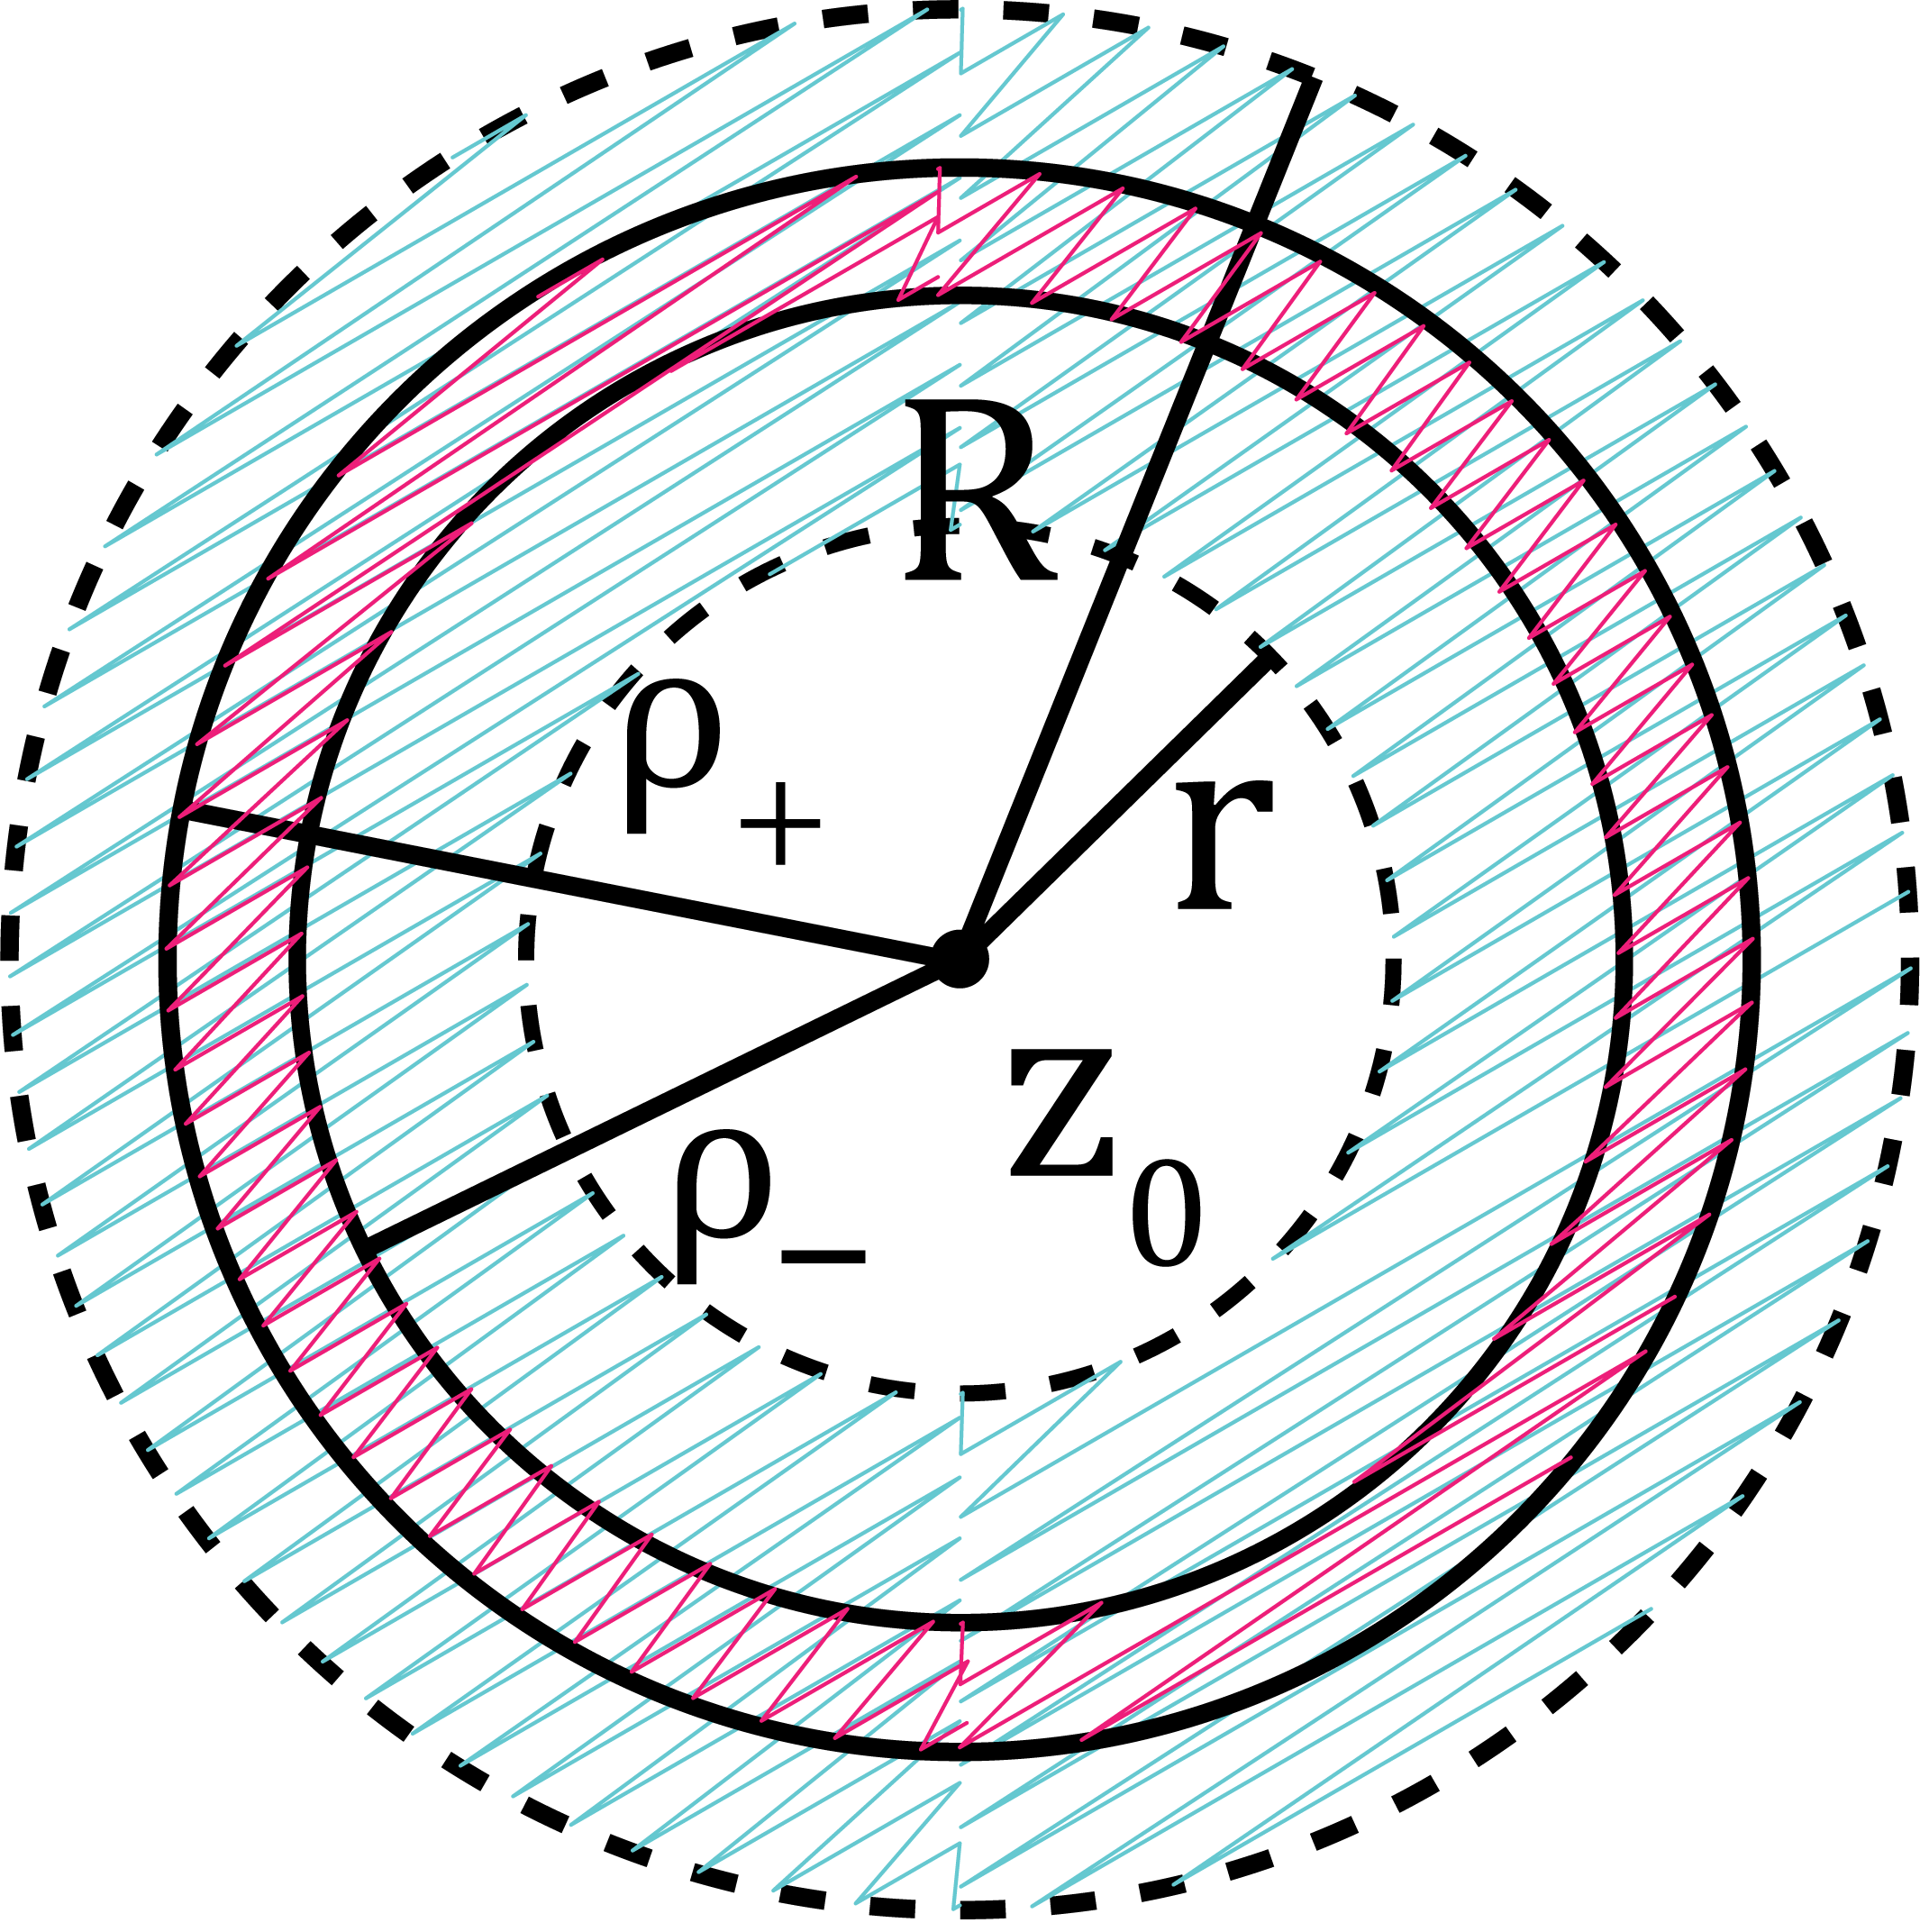
\includegraphics[width=5cm]{pics/12_11}
            \centering
        \end{figure}

        \[\forall \rho_+, \rho_-: \q r < \rho_- \leq \rho_+ < R\]
        \[\Ra \text{в кольце } \overline{K} = \{z : \rho_- \leq \abs{z - z_0} \leq \rho_+\}\]
        \[\text{Сх-ть ряда Л. равномерна} \q \text{(УПР)}\]
    \end{Definition}

    \begin{Theorem}[о разл. в р. Лорана]
        \[z_0 = 0,\q K = \{z : \ r < \abs{z} < R\}\]
        \[f \in H(K) \RA f(z) = \sum_{k = -\infty}^\infty c_k \cdot z^k \text{ --- р. Лорана} \]
        \[\text{Сх. равномерно в кольце } \rho_- \leq \abs{z} \leq \rho_+ \qq \forall r < \rho_- \leq \rho_+ < R\]
        \[c_k = \frac{1}{2\pi i}\int_{\gamma_{\rho}}  \frac{f(\xi)}{\xi^{k + 1} }d\xi \qq
        r < \rho < R\]
    \end{Theorem}

    \begin{Proof}
        %рисунок12
        \begin{figure}[H]
            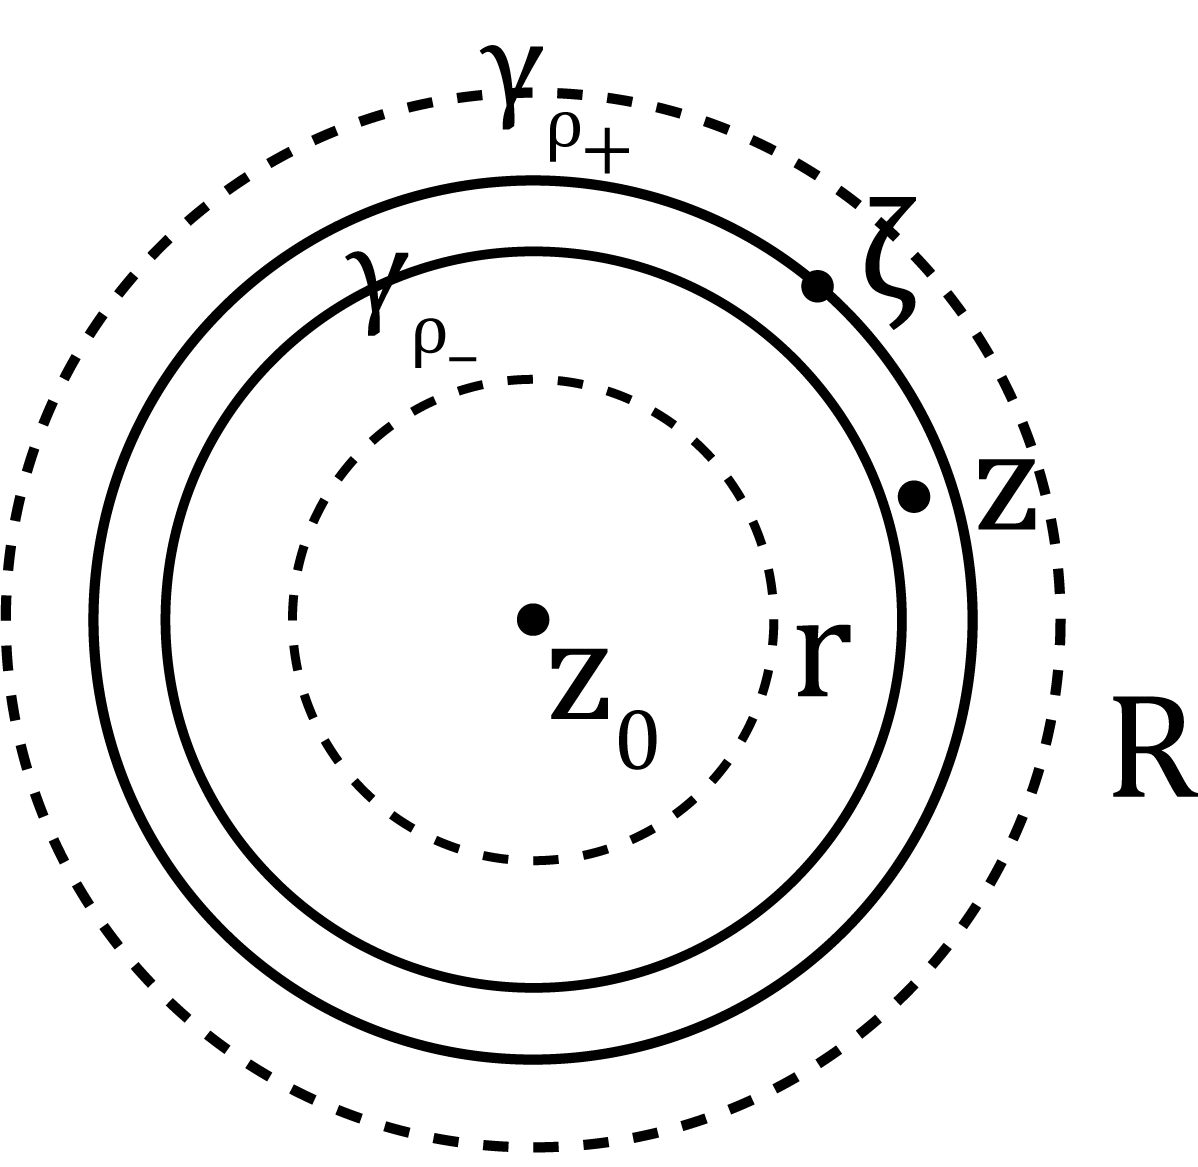
\includegraphics[width=5cm]{pics/12_12}
            \centering
        \end{figure}

        \[r < \abs{z} < R\]
        \[\letus r < \rho_- < \abs{z} < \rho_+ < R\]
        Инт. ф. Коши
        \[f(z) = \frac{1}{2\pi i} \left(\int_{\us{\text{пр. ч.с}}{\gamma^+_{\rho^+}} \cup
        \us{\text{по ч.с}}{\gamma^-_{\rho^-}}  } \frac{f(\xi)}{\xi - z}d\xi \right)\]
        \[\frac{1}{2\pi i} \int_{\gamma_{\rho^+} } \frac{f(\xi)}{\xi - z}d\xi - \frac{1}{2\pi i}
        \int_{\gamma_{\rho_-} } \frac{f(\xi)}{\xi - z} d\xi = f^+(z) - f^-(z) \]
        \[f^+(z) =  \frac{1}{2\pi i} \int_{\gamma_{\rho^+} }  \frac{f(\xi)}{\xi - z} d\xi = \]
        \[\rho^- < \abs{z} < \abs{\xi} = \rho^+\]
        \[= \frac{1}{2\pi i}\int_{\gamma_{\rho^+} } \frac{f(\xi)}{\xi} \frac{1}{1 - \frac{z}{\xi}} d\xi \os{\abs{\frac{z}{\xi}} < 1}{=}  \frac{1}{2\pi i} \int_{\gamma_{\rho_+} } \frac{f(\xi)}{\xi} \sum_{k = 0}^\infty
        \left(\frac{z}{\xi}\right)^k d\xi\]
        \begin{figure}[H]
            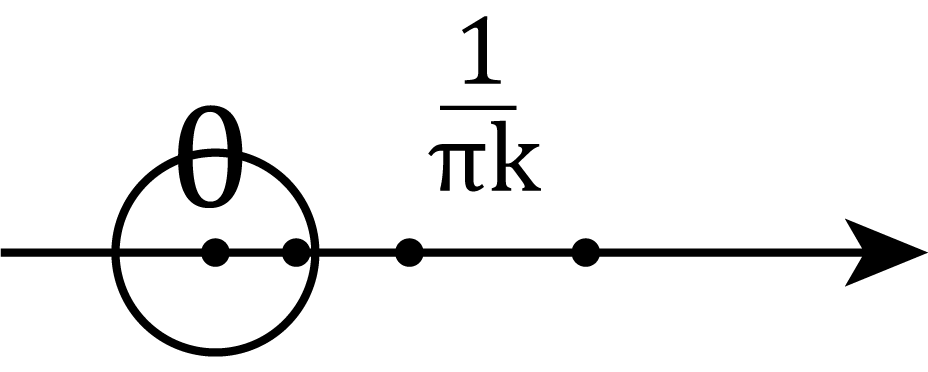
\includegraphics[width=5cm]{pics/12_14}
            \centering
        \end{figure}
        По пр. Вейерштрасса ряд сх. равномерно $\Ra $ можно инт.
        \[\Ra \frac{1}{2\pi i} \sum_{k = 0}^\infty z^k \int_{\gamma_{\rho^+}} \frac{d(\xi)}{\xi^{k+1}} d\xi\]
        \[f^-(z) = \frac{1}{2\pi i} \int_{\gamma_{\rho^-}} \frac{f(\xi)}{\xi - z} d \xi = \frac{1}{2\pi i} \int_{\gamma_{\rho^-}} \frac{f(\xi)}{z} \us{\text{ --- геом. прогр. } \abs{\frac{\xi}{z}} < 1}{\frac{1}{\frac{\xi}{z} - 1} d\xi} = \]
        \[= - \frac{1}{2\pi i} \int_{\gamma_{\rho^-}} \frac{f(\xi)}{z} \sum_{k=0}^{\infty} \frac{\xi^k}{z^k} d\xi \us{\text{на }\gamma_{\rho^-}}{\os{\text{ряд сх. равн.}}{=}} - \frac{1}{2 \pi i} \sum_{k=0}^{\infty} z^{-k-1} \int_{\gamma_{\rho^-}} f(\xi) \xi^k d\xi =\]
        \[= - \frac{1}{2\pi i} \sum_{n=-1}^{-\infty} z^n \int_{\gamma_{\rho^-}} \frac{f(\xi)}{\xi^{n+1}} d\xi\]
        \[f(z) = f^+ - f^- = \frac{1}{2\pi i} \sum_{k=0}^{\infty} z^k \int_{\gamma_{\rho^+}} \frac{f(\xi)}{\xi^{k+1}} d\xi + \frac{1}{2\pi i} \sum_{k=-1}^{-\infty} z^k \int_{\gamma_{\rho^-}} \frac{f(\xi)}{\xi^{k+1}} d\xi\]
        \[\forall \rho_1, \rho_2 \in (r, R)\]
        \[\int_{\gamma_{\rho_1}} \frac{f(\xi)}{\xi^{k+1}} d\xi = \int_{\gamma_{\rho_2}} \frac{f(\xi)}{\xi^{k+1}} d\xi\]
        Значит инт. не зависит от $\rho$!
        \[f(z) = \sum_{-\infty}^{+\infty} c_k z^k \q r < \rho < R\q c_k = \frac{1}{2 \pi i} \int_{\gamma_{\rho}} \frac{f(\xi)}{\xi^{k+1}} d\xi\]
    \end{Proof}
\end{document}
